
\documentclass[12pt]{amsart}
\usepackage{amssymb,amsmath}
\usepackage{graphicx}
\usepackage{geometry} % see geometry.pdf on how to lay out the page. There's lots.
\geometry{a4paper} % or letter or a5paper or ... etc
% \geometry{landscape} % rotated page geometry

% See the ``Article customise'' template for come common customisations

\title{Visualizing Grover's Search Algorithm}
\author{James Weaver \& Paul Kassebaum}
\date{} % delete this line to display the current date

%%% BEGIN DOCUMENT
\begin{document}

\maketitle

\section{How Grover's Works}

If we want an operator $U_x$ with the following behavior

\begin{equation}
	\begin{split}
		U_x |x\rangle & = - |x\rangle \\
		U_x |y\rangle & = |y\rangle 
	\end{split}
\end{equation}

where all $|y\rangle$ are orthogonal to $|x\rangle$, then the operator takes the form

\begin{equation}
	U_x = I - 2 |x\rangle\langle x|
\end{equation}

Let's demonstrate this with a couple of examples.

\begin{equation}
	\begin{split}
		U_x |x\rangle & = (I - 2 |x\rangle\langle x| ) |x\rangle \\
		& = |x\rangle - 2 |x\rangle\langle x | x\rangle \\
		& = |x\rangle - 2 |x\rangle \\
		& = - |x\rangle
	\end{split}
\end{equation}

because $\langle x | x\rangle = 1$.

\begin{equation}
	\begin{split}
		U_x |y\rangle & = (I - 2 |x\rangle\langle x| ) |y\rangle \\
		& = |y\rangle - 2 |x\rangle\langle x | y\rangle \\
		& = |y\rangle - 2 \langle x | y\rangle  |y\rangle \\
		& = |y\rangle
	\end{split}
\end{equation}

because $\langle x | y\rangle = 0$.

Now let's look at the result of acting on an arbitrary state $|\alpha\rangle$, that is not completely orthogonal to $|x\rangle$.

\begin{equation}
	\begin{split}
		U_x |\alpha\rangle & = (I - 2 |x\rangle\langle x| ) |\alpha\rangle \\
		& = |\alpha\rangle - 2 |x\rangle\langle x | \alpha\rangle \\
		& = (1 - 2 \langle x | \alpha\rangle)  |\alpha\rangle \\
	\end{split}
\end{equation}

In words, the result is the original state vector minus twice the overlap or projection of $|\alpha\rangle$ on $|x\rangle$. We can draw this out geometrically.
\begin{figure}[h]
   \centering
   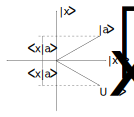
\includegraphics[width=0.5\textwidth]{./img/fig-00} % requires the graphicx package
   \caption{Geometric demonstration that the operator $U_x$ has the effect of reflecting $|\alpha\rangle$ across $|x_\perp\rangle$, the vector orthogonal to $|x\rangle$.}
   \label{fig:example}
\end{figure}

\end{document}